\usection{Il gioco a grandi linee}

Come ogni manuale ti dirà, \dnd{} ha un \textbf{arbitro} (Dungeon Master, Game Master) e un po' di giocatori. L'arbitro prepara uno scenario, un'avventura da vivere, mentre i giocatori preparano un gruppo di avventurieri per superare quello scenario. Fino a qui tutto bene, è l'immagine a grandi linee.

Andando più a fondo, la virtù dell'avventura, quello che ci piace nel gioco, sta nelle sue \textbf{qualità letterarie} che suggeriscono temi accessibili e importanti per gli esseri umani: avventura, storia, fantasia. Il concetto è che il gioco dovrebbe presentare, affrontare e permettere che queste cose vengano esperite. Il gioco parla di queste qualità letterarie nel senso che ne formano l'argomento sostanziale: \dnd parla di eserciti medievali, draghi, elfi e maghi. Queste cose possono essere sperimentate e ci si può interagire in gioco.

Quindi, qual è lo scopo del gioco? Scegliendo quella che per alcuni è la prima risposta mai data a questa domanda - dipende da in che punto della storia si posizionano i giochi di ruolo terapeutici, suppongo - la via del \textit{wargaming} sostiene che dobbiamo plasmare \textbf{sfide} ed enigmi usando la sostanza della narrazione e porci l'un l'altro queste sfide, scenari o avventure. Lottando, dibattendo e superando le difficoltà ci godiamo l'argomento perché lo apprendiamo in maniera pratica: la prospettiva in prima persona, che è caratteristica di tutte le arti ludiche, ci permette di immergerci ben oltre i gomiti nel materiale.

\usubsection{I duplici meriti della pratica}

Mentre l'arbitro offre scenari perché vengano considerati da un punto di vista da \textit{wargamin}, il compito dei giocatori è di affrontare la situazione, pensare e decidere, spiegare il loro ragionamento ed eseguire un piano che guidi lo scenario verso la vittoria per la fazione che gli è stata assegnata. Specificamente in \dnd{}, i giocatori pilotano ciascuno un singolo personaggio, formando un gruppo di avventurieri che affronta unito lo scenario dell'arbitro.

Questa attività di \wargam{ing} ha i meriti dello sport: pratichiamo completamente la \textbf{sportività}, dalle relazioni sociali delle squadre e delle rivalità alla costruzione del carattere data da vittorie e sconfitte. Ha anche i meriti dell'\textbf{istruttività}: quale che sia l'argomento del gioco, il \wargam{er} lo impara a fondo, lo mette alla prova con gli strumenti della simulazione e ha il potenziale di derivarne conoscenza su come funzionano le cose.

La chiave per un gioco più intenzionale sta nel capire cosa lo rende soddisfacente in prima battuta. Sportività e istruttività, questi sono gli scopi creativi della via del \wargam{ing}.

\begin{figure}[p!]
    \resizebox{\linewidth}{!}{
        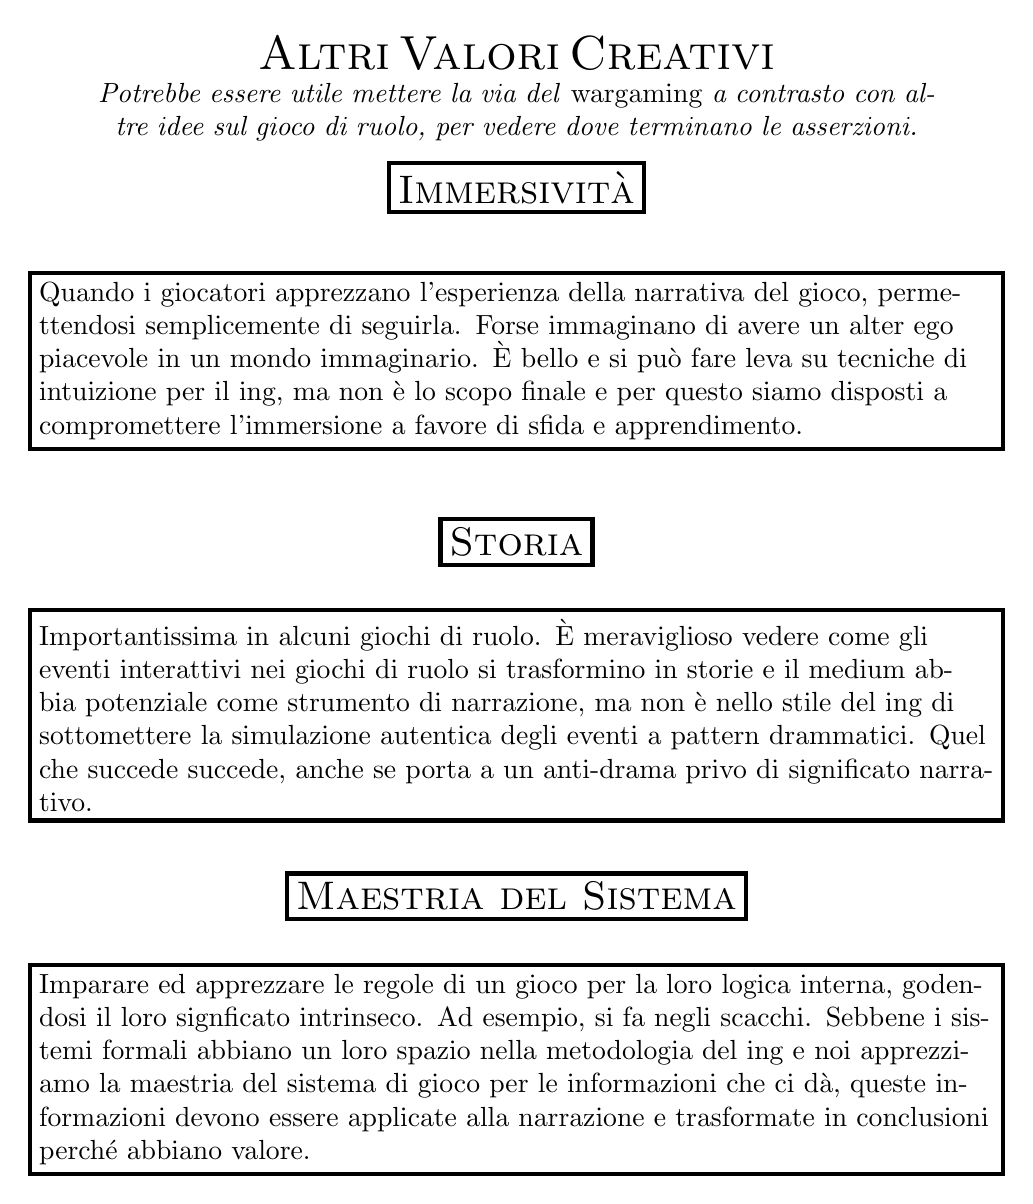
\begin{tikzpicture}
            \node[text width=\linewidth, align=center] (T) at (-1, 0.25) {
                    \textsc{\LARGE{Altri Valori Creativi}}\\
                    \textit{Potrebbe essere utile mettere la via del} wargaming \textit{a contrasto con altre idee sul gioco di ruolo, per vedere dove terminano le asserzioni.}
                };

            \node[draw, ultra thick, rectangle,font=\Large\scshape] (A) at (-1, -1) {Immersività};
            \node[draw, ultra thick, rectangle, text width=\linewidth] at (-1, -3.2) {
                Quando i giocatori apprezzano l'esperienza della narrativa del gioco, permettendosi semplicemente di seguirla. Forse immaginano di avere un alter ego piacevole in un mondo immaginario. È bello e si può fare leva su tecniche di intuizione per il \wargam{ing}, ma non è lo scopo finale e per questo siamo disposti a compromettere l'immersione a favore di sfida e apprendimento.
            };

            \node[draw, ultra thick, rectangle,font=\Large\scshape] (A) at (-1, -5.5) {Storia};
            \node[draw, ultra thick, rectangle, text width=\linewidth] at (-1, -7.7) {
                Importantissima in alcuni giochi di ruolo. È meraviglioso vedere come gli eventi interattivi nei giochi di ruolo si trasformino in storie e il medium abbia potenziale come strumento di narrazione, ma non è nello stile del \wargam{ing} di sottomettere la simulazione autentica degli eventi a pattern drammatici. Quel che succede succede, anche se porta a un anti-drama privo di significato narrativo.
            };

            \node[draw, ultra thick, rectangle,font=\Large\scshape] (A) at (-1, -10) {Maestria del Sistema};
            \node[draw, ultra thick, rectangle, text width=\linewidth] at (-1, -12.2) {
                Imparare ed apprezzare le regole di un gioco per la loro logica interna, godendosi il loro signficato intrinseco. Ad esempio, si fa negli scacchi. Sebbene i sistemi formali abbiano un loro spazio nella metodologia del \wargam{ing} e noi apprezziamo la maestria del sistema di gioco per le informazioni che ci dà, queste informazioni devono essere applicate alla narrazione e trasformate in conclusioni perché abbiano valore.
            };
            
        \end{tikzpicture}
    }
\end{figure}

\usubsection{Consigli di lettura}

Prendi un qualsiasi manuale di \dnd{} vecchia scuola come punto di partenza. Non importa quale di preciso; il gioco ha una storia creativa rudimentale e i suoi testi tendono a danzare attorno agli scopi essenziali. Piuttosto agli inizi, nei primi anni '80, i testi cominciano a incoraggiare una comprensione del gioco che è più orientata verso l'eccitante esperienza di essere un avventuriero fantasy e meno verso il \wargam{e}. Anche così, tuttavia, non si tratta di un ostacolo essenziale, perché le regole effettive e la struttura del gioco sopravvivono per un po'.

Fai riferimento al tuo manuale in parallelo a questo studio. Troverai che il testo descrive delle procedure e meccaniche di gioco per creare e far salire di livello degli avventurieri fantasy. C'è una sezione di regole di combattimento per risolvere piccole schermaglie tra avventurieri e mostri. Sperabilmente, c'è una serie di "regole per l'esplorazione del dungeon", le procedure di esplorazione di un labirinto sotterraneo.

Tutta questa materia regolistica alla fine esiste al servizio della più alta idea di simulazione di manovre avventurose contro un'opposizione dinamica in un ambiente fantastico. I particolari di come le regole lo facciano sono talvolta piuttosto intelligenti, ma non me ne preoccupo particolarmente qui; è più importante che i giocatori si confrontino con un puzzle, una sfida: data questa situazione fantastica, questo \textbf{scenario}, cosa sceglierà l'eroe, quale \textbf{manovra} ti porterà alla vittoria? Questa è la conversazione che stiamo facendo. Le regole ne sono semplicemente il linguaggio.

\usubsection{Regolamenti appropriati}

Molte persone non esiterebbero a chiamare ciò che insegno qui "\dnd{} vecchia scuola". Va bene, io stesso uso questo termine quando aiuta più di quanto non saboti. Il motivo per cui non lo metto così in evidenza è che non voglio appropriarmi di un'etichetta che ha sensibilità culturali ancora più ampie: ci sono certamente dei giocatori di \dnd{} vecchia scuola che non concorderebbero con ciò che sto presentando qui; voglio rispettare questo disaccordo. "Vecchia scuola" si riferisce alla più vasta cultura di ciò che \dnd{} era negli anni '70 e, sebbene io pensi che sia corretto considerare Muster \textit{una descrizione particolare} di quel momento, ci sono anche altre dottrine "old school" là fuori che sono incompatibili.

Detto questo, se si cercano regolamenti genericamente compatibili con Muster, qualsiasi cosa sia identificato come "old school" funzionerà probabilmente meglio di qualsiasi cosa più moderna. I cambiamenti incrementali e un paio di rivoluzioni nella cultura di \dnd{} dagli anni '70 ad oggi causano un disordine inutile da districare per chi stia cominciando. Per motivi pratici, prendi un qualsiasi testo della "vecchia scuola" come punto di partenza.

Non considero la scelta di uno specifico testo di regole come essenziale per giocare nello stile \wargam{ing}. Potresti persino prendere la più recente edizione di \dnd{}, la 5° al momento in cui sto scrivendo, e applicare il tuo stile di gioco a quella. Si fa solo più fatica.

Alla fin fine, la scelta dovrebbe dipendere esclusivamente sul fatto che l'\textbf{estetica delle meccaniche} ti piaccia o meno e su quanto bene lo scheletro delle regole si applichi all'\textbf{argomento della tua campagna} in senso simulativo. Aiuta anche se il testo delle regole non milita attivamente contro lo stile \wargam{ing}, ma sta a te decidere quanta lettura critica e riorganizzazione iniziale ti senti di fare.

Per essere chiari: qualsiasi testo tu scelga, può essere solamente un punto di partenza. Scegli un punto di partenza con cui ti sembri piacevole lavorare, ma non trasformare il "sistema" in un oggetto di culto. La via del \wargam{ing} prevede di contaminarlo con la realtà dei \textit{ruling} che verranno, specifici per ogni campagna.

\usection{Le Regole sono Semplici e Rozze}

Affronterò una reazione piuttosto ovvia, che molte persone hanno quando incontrano \dnd{} per la prima volta. Questo è ancora più vero per i giocatori che hanno imparato inizialmente con altri giochi, come me.

Questa prima reazione alla lettura del testo delle regole è che le regole appaiano tanto \textbf{semplici} quanto \textbf{rozze} se paragonate ad altri giochi. Il conservatorismo tecnico ha dominato le prime tre decadi della cultura di \dnd{}, che è una brutta situazione in cui trovarsi se stai anche sviluppando cose nuove e, di conseguenza, attraversando fasi di design strane e rozze.

Per esempio, difficilmente troverai un sistema di regole per le abilità, elaborato e degno di questo nome, in qualsiasi regolamento di \dnd{}. E se dovessi farlo, sarà piuttosto rozzo e primitivo. E comunque impiegherà numerose pagine dense di regole e testo, riuscendo contemporaneamente a risultare semplice e complicato.

Ricordo molto bene quale fosse la mia prospettiva su \dnd{} negli anni '90, da adolescente che stava familiarizzando coi giochi di ruolo. Ai tempi non era raro che i giocatori finlandesi venissero cresciuti esclusivamente con una dieta di giochi tradizionali post-\dnd{}, come \textsc{Runequest}, \textsc{Paranoia}, e \textsc{Cyberpunk 2020}, una ricca vena di giochi \textit{mainstream}\dots ma priva dell'egemonia di \dnd{} tipica dell'esperienza americana.

\begin{figure}[p!]
    \resizebox{\linewidth}{!}{
        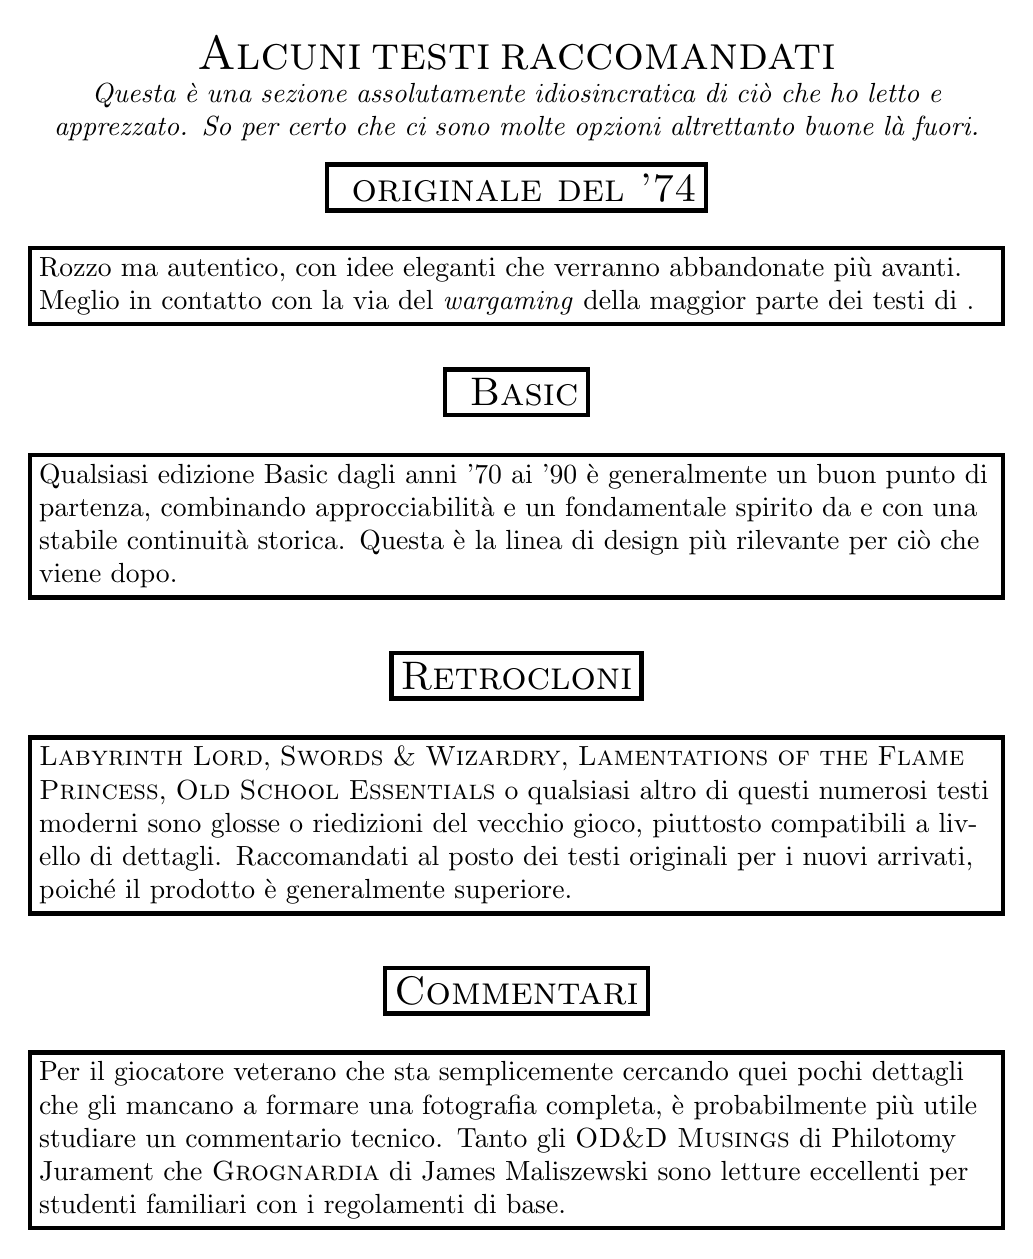
\begin{tikzpicture}
            \node[text width=\linewidth, align=center] (T) at (-1, 0.25) {
                    \textsc{\LARGE{Alcuni testi raccomandati}}\\
                    \textit{Questa è una sezione assolutamente idiosincratica di ciò che ho letto e apprezzato. So per certo che ci sono molte opzioni altrettanto buone là fuori.}
                };

            \node[draw, ultra thick, rectangle,font=\Large\scshape] (A) at (-1, -1) {\dnd{} originale del '74};
            \node[draw, ultra thick, rectangle, text width=\linewidth] at (-1, -2.25) {
                Rozzo ma autentico, con idee eleganti che verranno abbandonate più avanti. Meglio in contatto con la via del \textit{wargaming} della maggior parte dei testi di \dnd{}.
            };

            \node[draw, ultra thick, rectangle,font=\Large\scshape] (A) at (-1, -3.6) {\dnd{} Basic};
            \node[draw, ultra thick, rectangle, text width=\linewidth] at (-1, -5.3) {
                Qualsiasi edizione Basic dagli anni '70 ai '90 è generalmente un buon punto di partenza, combinando approcciabilità e un fondamentale spirito da \wargam{e} con una stabile continuità storica. Questa è la linea di design più rilevante per ciò che viene dopo.
            };

            \node[draw, ultra thick, rectangle,font=\Large\scshape] (A) at (-1, -7.2) {Retrocloni};
            \node[draw, ultra thick, rectangle, text width=\linewidth] at (-1, -9.1) {
                \textsc{Labyrinth Lord}, \textsc{Swords \& Wizardry}, \textsc{Lamentations of the Flame Princess}, \textsc{Old School Essentials} o qualsiasi altro di questi numerosi testi moderni sono glosse o riedizioni del vecchio gioco, piuttosto compatibili a livello di dettagli. Raccomandati al posto dei testi originali per i nuovi arrivati, poiché il prodotto è generalmente superiore.
            };

            \node[draw, ultra thick, rectangle,font=\Large\scshape] (A) at (-1, -11.2) {Commentari};
            \node[draw, ultra thick, rectangle, text width=\linewidth] at (-1, -13.1) {
                Per il giocatore veterano che sta semplicemente cercando quei pochi dettagli che gli mancano a formare una fotografia completa, è probabilmente più utile studiare un commentario tecnico. Tanto gli \textsc{OD\&D Musings} di Philotomy Jurament che \textsc{Grognardia} di James Maliszewski sono letture eccellenti per studenti familiari con i regolamenti di base.
            };
            
        \end{tikzpicture}
    }
\end{figure}

Quando quell'adolescente, cresciuto con una tradizione di GDR matura e post-\dnd{} incontrava \dnd{} (nel mio caso, nella forma del Basic di Mentzer e di A\dnd{} 2e), il gioco era quasi incomprensibile. E non era semplicemente perché mi mancava il contesto creativo per capire come un gioco di ruolo potesse mai essere un \textit{wargame}; no, addirittura ero più confuso da quanto rozzo e caotico fosse il gioco dal punto di vista tecnico. Mancare completamente l'idea della sfida posta non aiutava, ovviamente, ma non importa; questi non erano affatto i migliori regolamenti per i criteri dell'epoca.

È tutto vero, ma con un po' più di esperienza sulle spalle credo di poter spiegare il perché di questa situazione. Questa spiegazione potrebbe esserci utile per costruire un po' di fiducia; dovresti mettere alla prova il gioco secondo i suoi meriti, prima di condannarlo per non aver rispettato i criteri di giochi successivi, costruiti senza tenere a mente la via del \wargam{ing}.

\usubsection{Perché essere semplici}

Essenzialmente, le regole di \dnd{} sono semplici perché si suppone che vengano utilizzate in brevi e atomizzate catene formali di meccaniche, che si ricollegano costantemente alla situazione fittizia di cui i giocatori stanno tenendo traccia con le loro menti, mappe e pedine. Le regole devono sopravvivere allo stress di permettere alla narrazione di svilupparsi organicamente. La successiva tradizione del gioco di ruolo ha il lusso di aver scartato questo requisito di applicabilità generica in favore di considerazioni fisse su scenari stabili: puoi permetterti di costruire cose più elaborate se hai preconcetti più forti riguardo a cosa sarà il gioco. Fondamentalmente, le scene teatrali possono permettersi dettagli formali più complessi rispetto alla vera interpretazione.

Credo che l'esempio più notevole di come questo principio di design influenzi le prestazioni del gioco stia nel modo in cui \dnd{} è capace di valutare azioni di schermaglia \textit{con grossi input dinamici}. Una campagna di \dnd{} ben sviluppata contiene manovre operative autentiche, che conducono a battaglie letali e dalla posta altissima con una gran varietà di nature, dagli assedi agli inseguimenti, \textit{completamente in tempo reale}. Puoi risolvere 20 schermaglio nel tempo in cui molti giochi nuovi ne risolvono una, il tutto senza preparazioni prima della sessione.

Un altro esempio piuttosto chiaro è la creazione del personaggio, qualcosa che è diventato l'attività primaria e di estrema complessità in alcune branche del GdR moderno. Il processo usato nei primi \dnd{} è molto più semplice, ma ricorda che era inteso per un gioco autenticamente ad alta letalità, dove davvero \textit{era possibile} perdere il personaggio a un quarto d'ora dall'inizio della partita. Quanto sarebbe stato piacevole combinare un \textit{progetto} di creazione del personaggio che fosse pesante e meditativo con quel tipo di gioco?

Questa non è una proprietà triviale per un gioco di ruolo di avventura fantasy. Le iterazioni successive della stessa forma falliscono sistematicamente, perché non sono atomicamente semplici nelle loro rispettive regole per fare le stesse cose. Puoi, più o meno, simulare la semplicità ignorando le regole, ma non è la stessa cosa.

\usubsection{Perché essere rozzi}

Ma quindi, se le regole sono volutamente semplici, perché sono così rozze? Ho studiato la tradizione testuale di \dnd{} per un bel po' e ammetto candidamente che i testi del gioco cominciano davvero ad avere senso solo dopo la caduta della TSR; fino a quel momento cominciano come improvvisazioni dilettantesche, si evolvono in follia da venditori di olio di serpente e sprofondano in meschinità aziendale. Sto solo dicendo cosa vedo, eh.

Chiaramente, non è detto che le regole \textit{debbano} essere rozze, anche se è quello che sembrava negli anni '80. Sviluppi paralleli nell'industria del gioco, tanto nel \wargam{ing} che nel gioco di ruolo, non hanno avuto questi problemi.

La motivazione principale di questa situazione rimanda alla natura dei \textbf{residuati regolistici}\translatornote{Vedi le considerazioni su "cruft" in \hyperref[notes:cruft]{nota a pagina \pageref*{notes:cruft}}}. I primi testi di \dnd{} sono per loro stessa natura una trascrizione molto cruda di quello che sembra essere l'autentico processo di gioco degli autori. Sebbene non ci sia nulla in particolare che impedisca di assemblare regole più logiche, snelle e realizzate ad arte per supportate il gioco, i primi testi basilari\translatornote{Le prime edizioni di \dnd{} dividevano i manuali in "basic", che coprivano i primi livelli di gioco, e diverse altre categorie che coprivano altre fasce. Credo che il riferimento qua sia tanto alla semplicità quanto a quella categoria di manuali.} non sono così: sono trascrizioni piuttosto amatoriali e, ed è peggio, sono stati compilati con l'erronea convinzione che il pubblico avesse un disperato bisogno di queste dettagliate e minute spiegazioni delle regole usate al tavolo della campagna origianel. I testi cercano di trapiantare l'intera campagna dal gruppo dell'autore al vostro, invece di concentrarsi su come coltivare la vostra.

Per via di come funzionano i residuati regolistici, una \textbf{struttura adeguata} è necessaria per il loro uso effettivo: quali che siano le regole che usi, dovresti conoscerle a memoria e supportartle come il materiale che hai scelto per la tua campagna. Questo requisito di usabilità interagisce molto male con la tradizione testuale di trascrivere centinaia e centinaia di pagine di minuzie. Non è che le regole non avrebbero davvero funzionato nella campagna da cui derivano, ma quella campagna aveva un arbitro estremamente versato nel materiale e che lo stava applicando al mondo di gioco da cui quelle regole nascevano. Ed è persino possibile che un gruppo successivo studi quei residuati regolistici finché non ne diventano una seconda natura. Ma non dovresti farlo, perché è veramente tanto sforzo per poco beneficio.

La rozzezza generale dei testi regolistici originali è innegabile nonostante contengano diverse perle di comprensione del game design. Quello che salva il gioco nella sua totalità è che \textbf{non hai alcun dovere nei confronti di tutti quei residuati regolistici}. Il gioco non sono i residuati, ma la struttura sottostante. Se in certi punti le regole ti sembrano rozze, come succede a me, rimpiazzale con altre più eleganti. Stiamo in piedi sulle spalle di giganti, \textit{dovremmo} essere in grado di migliorare i primi tentativi di residuati regolistici per giochi di ruolo di avventura fantasy.

È interessante notare come, quando Internet prese piede e la soppressione aziendale delle pubblicazioni accademiche su \dnd dell'era della TSR si allentò un poco, quello che divenne rapidamente evidente era che il gioco, com'era praticato dai singoli master in giro per il mondo, non era affatto rozzo! Raccomando di leggere le procedure e meccaniche usate effettivamente da arbitri esperti e capaci, che scelgano di pubblicare le loro \textit{house rules} in forma di libro o meno. Sono quasi senza eccezione molto, molto più eleganti, efficienti, comprensibili e rilevanti per le campagne degli originali storici o del pastone aziendale che la TSR ne ha ricavato nel corso degli anni 80. È un mondo completamente diverso.

Questo potrebbe sembrare ovvio ad alcuni, ma la storia testuale di \dnd{} ha sempre posseduto un forte tratto di una cultura "solo regole ufficiali". Quindi considera il mio contrappunto: le regole ufficiali non sono così fighe, non credere ai venditori ambulanti. Leggi criticamente, puoi migliorarle e costruirci su una campagna migliore.